\documentclass{article}

% Chinese Support using xeCJK
% \usepackage{xeCJK}
% \setCJKmainfont{SimSun}

% Chinese Support using CTeX
\usepackage{ctex}

% Math Support
\usepackage{amsmath}
\usepackage{amsfonts}
\usepackage{amssymb}
\usepackage{wasysym}
\newcommand{\angstrom}{\text{\normalfont\AA}}
\usepackage{fancyhdr}

% Graphics Support
\usepackage{graphicx}
\usepackage{float}
\restylefloat{table}

% Reduced page margin
\usepackage{geometry}
\geometry{a4paper,scale=0.8}

\usepackage{caption}
\usepackage{subcaption}

% d and e should be math operators
\newcommand*{\dif}{\mathop{}\!\mathrm{d}}
\newcommand*{\md}{\mathop{}\!\mathrm{d}}
\newcommand*{\me}{\mathrm{e}}

% No indent for each paragraph
% \usepackage{parskip}
% \setlength{\parindent}{0cm}

% Bold style for Greek letters
\usepackage{bm}
\let\Oldmathbf\mathbf
\renewcommand{\mathbf}[1]{\boldsymbol{\Oldmathbf{#1}}}

% More space for dfrac in cell
\usepackage{cellspace}
\setlength{\cellspacetoplimit}{5pt}
\setlength{\cellspacebottomlimit}{5pt}

% SI units
\newcommand{\si}[1]{\  \mathrm{#1}}

% Multi-line author information
\usepackage{authblk}
\author{物理(4+4)1801 \quad  胡喜平 \quad U201811966}
\affil{个人网站 https://hxp.plus/ \quad 电子邮件 hxp201406@gmail.com}

\title{综合物理实验预习笔记——综合光学实验}

\pagestyle{fancy}
\fancyhf{}
\lhead{源码地址:https://github.com/hxp-plus/Notes/tree/master/Physics-Experiment}
\rfoot{第 \thepage 页}
\renewcommand{\headrulewidth}{1pt}
\renewcommand{\footrulewidth}{1pt}

\begin{document}

\maketitle\thispagestyle{fancy}

\section{实验内容}

\begin{itemize}
\item 测量励磁线圈的电流$I$和励磁线圈产生的磁场$B$之间的关系。
\item 测量法拉第磁光效应中磁致旋转角$\Delta \varphi$和磁场强度$B$的关系。
\item 测量LED的I-V特性和I-P特性。
\item 测量LED的I-V特性和I-P特性的温度效应。
\end{itemize}

\section{实验原理}

\subsection{法拉第磁光效应}

线偏振光透过放置于磁场中的物质,且沿着磁场方向传播时,光的偏振方向会发生变化。其中变化的角度,即法拉第旋转角,和样品长度$l$的关系为

\begin{equation*}
  \begin{aligned}
    \Delta \varphi = BlV
  \end{aligned}
\end{equation*}

其中$V$是与物质性质和光的频率有关的常数。其中测量法拉第旋转角的方法是不停旋转检偏镜,然后测量光强,绘制检偏镜角度和光强的角度。

\begin{figure}[H]
  \centering
  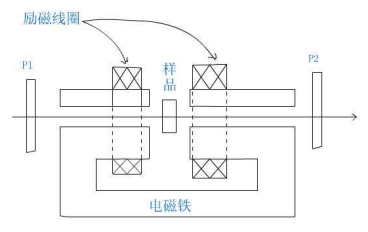
\includegraphics[width=0.5\linewidth]{figures/法拉第磁光效应}
  \caption{法拉第磁光效应}
  \label{fig:法拉第磁光效应}
\end{figure}

\subsection{LED的物理特性}

LED是一种半导体二极管,当PN结加入反向电压时,少数载流子难以注入,不发光而且电阻很大。当PN结加入正想电压时,电流从阳极流向阴级时,半导体内部注入的少数载流子和多数载流子复合时,会把多余的能量以光的形式释放出去,发出相应波长的光。

半导体的V-I特性和P-I特性应该是下图所示

\begin{figure}[H]
  \centering
  \begin{subfigure}{.45\textwidth}
    \centering
    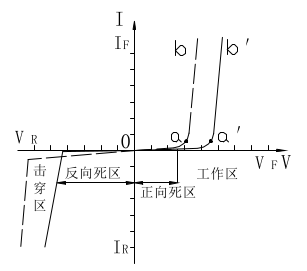
\includegraphics[width=\linewidth]{figures/LED的V-I特性}
    \subcaption{LED的V-I特性}
  \end{subfigure}
  \begin{subfigure}{.45\textwidth}
    \centering
    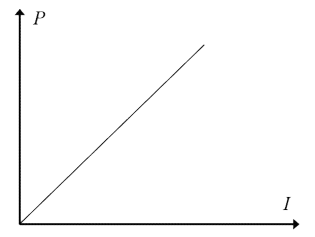
\includegraphics[width=\linewidth]{figures/LED的P-I特性}
    \subcaption{LED的P-I特性}
  \end{subfigure}
\end{figure}



\end{document} 
